\chapter{General relativity}


\section{The logical foundation of general relativity}
Like any physical theory, general relativity theory 
as a logical construct has precisely defined axioms that are assumed
and from which all other laws and properties can be deduced.
The essential axiom of general relativity theory is
the equivalence principle. 
%We will formulate it immediately in its
%heuristic form; for the strict mathematical
%formulation, please refer to \cite{Straumann-1988}.
Einstein elegantly formulated it in such a way that it “automatically”
implied two laws that he wanted to physically require from his
theory of gravity: the
correspondence principle and the equality of inertial and gravitational
mass.
The “correspondence principle” refers to the relationship
between gravitational theory and special relativity theory and
states that
locally, i.e., on a small scale or 
in areas of weak gravity, the laws of special relativity theory apply approximately.
In this way, general relativity theory contains
special relativity as a limiting case, because with vanishing masses
and uniform motions of bodies they merge into one another
\cite[p. 266]{Born-2001}.

The equality of heavy and inertial mass, on the other hand, 
states that the weight of a body in a given 
gravitational field is always proportional to its inertial mass:
all bodies fall at the same speed in the same gravitational field
\cite[pp. 37, 269ff]{Born-2001},
for example, in the Earth's gravitational field at the Earth's surface with a uniform
acceleration $g = 9.81$ m/s$^2$.
Accordingly, one can decrease one's weight by accelerating in the opposite direction, and vice versa.
Today, when television images and video clips of freely floating
astronauts are familiar to everyone, this fact hardly surprises
anyone.
%%Even by the comparatively small effect of rotation of the Earth, a person with a mass of 75 kg weighs about 250 g less at the equator than at the poles \cite[§1.3.2]{Gerthsen-Meschede-2015}. % p. 22
%
%%
%\begin{quote}
%	[Ende Oktober, Anfang November 1907]
%	„wurde mir klar, daß alle Naturgesetze innerhalb des Rahmens der
%	Speziellen Relativitätstheorie behandelt werden können -- nur
%	nicht das Gravitationsgesetz. Ich wollte die Gründe dafür verstehen.
%	[\ldots]
%	Ich saß auf meinem Stuhl im Patentamt in Bern. Plötzlich hatte ich 
%	einen Einfall: Wenn sich eine Person im freien Fall befindet, wird
%	sie ihr eigenes Gewicht nicht spüren. Ich war verblüfft.
%	Dieses einfache Gedankenexperiment machte auf mich einen tiefen
%	Eindruck. Es führte mich zu einer Theorie der Gravitation.“
%
%	\hfill{Albert Einstein (1922), 
%	zitiert nach \cite[S. 343]{Foelsing-1993}}
%\end{quote}
%
%\begin{quote}
%	„Für einen Beobachter, der sich im freien Fall vom Dach seines
%	Hauses befindet, existiert -- zumindest in seiner unmittelbaren 
%	Umgebung -- kein Gravitationsfeld.“
%
%	\hfill{Albert Einstein (1920),
%	zitiert nach \cite[S. 344]{Foelsing-1993}}
%\end{quote}
%
%\noindent
%Fölsing betont, dass zu der damaligen Zeit die Gleichheit von träger und
%schwerer Masse den meisten Physikern gar nicht bewusst war
%und nur vereinzelt von kritischen Geistern wie Heinrich Hertz
%oder Ernst Mach analysiert worden war, wovon Einstein wusste.
%Was Einstein jedoch offenbar nicht wusste, war, dass der ungarische
%Physiker Loránd Eötvös bereits 1889 die Gleichheit von träger und schwerer
%Masse experimentell bis auf ein Verhältnis von $1:10^8$
%bestätigt hatte
%\cite[S. 345]{Foelsing-1993}.
%
%Einstein schloss aus dem Äquivalenzprinzip radikal, dass die
%Wirkung eines Gravitationsfeldes ganz prinzipiell nicht von einer 
%beschleunigten Bewegung unterschieden werden kann und dass die
%Geometrie einer Raumzeit mit einem Gravitationsfeld
%gekrümmt sein muss.
%Sein Gedankengang dabei war in etwa folgender.
%Nach den Gesetzen der speziellen Relativitätstheorie
%sind die Bahnen gleichförmig bewegter Körper und
%ebenso die Lichtstrahlen stets die kürzesten Linien zwischen
%zwei Raumzeitpunkten.
%Unbeschleunigte Bewegungen 
%im gravitationsfreien Raum beschreiben
%stets Geraden.
%In beschleunigten Bezugssystemen,
%oder äquivalent in Bezugssytemen in einem
%Gravitationsfeld,
%müssen dann aber die kürzesten Linien
%gekrümmt sein.
%Dieser Gedanke kam Einstein bereits 1907.
%Die folgenden acht Jahre bemühte er sich
%„nur“ noch darum, diese Idee mathematisch präzise
%zu auszuformulieren.
%
%%Mit einem einfachen Gedankenexperiment schloss Einstein
%%daraus und aus der Annahme der Gleichheit von träger und schwerer
%%Masse auf die Gekrümmtheit der Raumzeitgeometrie.
%
%%------------------------
%
%
%In seinem Vortrag "`Einiges über die Entstehung der allgemeinen Relativitätstheorie"'
%führte Einstein aus, wie er auf diese wesentlichen Erkenntnis 
%%zur Entwicklung seiner Gravitationstheorie 
%kam:
%
%\begin{quote}
%%\begin{em}
%	"`Ich kam der Lösung des Problems zum erstenmal einen Schritt näher, als
%	ich versuchte, das Gravitationsgesetz im Rahmen der speziellen
%	Relativitätstheorie zu behandeln. Wie die meisten damaligen Autoren
%	versuchte ich, ein Feldgesetz für die Gravitation aufzustellen,
%	da ja die Einführung unvermittelter Fernwirkung wegen der Abschaffung
%	des absoluten Gleichzeitigkeitsbegriffs nicht mehr [\ldots] möglich war.
%	[\ldots]
%	
%	Solche Überlegungen führten aber zu einem Ergebnis, das [\ldots]
%	nicht zur alten Erfahrung [passte], dass die Körper alle dieselbe
%	Beschleunigung in einem Gravitationsfeld erfahren. Dieser Satz, der
%	auch als der Satz von der Gleichheit der trägen und schweren Masse
%	formuliert werden kann, leuchtete mir nun in seiner tiefen Bedeutung
%	ein. Ich wunderte mich im höchsten Grade über sein Bestehen und vermutete,
%	dass in ihm der Schlüssel für ein tieferes Verständnis der Trägheit
%	und Gravitation liegen müsse.
%	[\ldots]
%	Nun verwarf ich den Versuch der oben angedeuteten Behandlung des
%	Gravitationsproblems im Rahmen der speziellen Relativitätstheorie
%	als inadäquat. Er wurde offenbar der fundamentalsten Eigenschaft
%	der Gravitation nicht gerecht."'
%%\end{em}
%
%	\hfill{zitiert nach \cite[S.~81f]{Straumann-1988}}
%\end{quote}
%
%
%
%\subsection{Das Äquivalenzprinzip}
%Gemäß Galilei fallen alle Körper unter Vernachlässigung des Luftwiderstands
%gleich schnell. 
%Die physikalische Grundlage f\"ur die allgemeine Relativit\"at ist die 
%experimentell bis
%auf eine Genauigkeit von $10^{-12}$ nachgewiesene
%Identit\"at von tr\"ager und schwerer Masse. Auf ihr
%beruht die Schwerelosigkeit in einer antriebslos fallenden Rakete, 
%denn Beschleunigung und Gravitation kompensieren sich durch diese 
%Identit\"at.
Regarding these two principles, Einstein unified them and formulated the now so-called Einstein equivalence principle:

\begin{axiom}[\textbf{Einstein equivalence principle}]
	\label{equivalence-principle}%
	\cite[S. 88]{Straumann-1988}
	No local experiments can distinguish a non-rotating system falling freely in a gravitational field (a “local inertial frame”) from a uniformly moving system in gravity-free space.
\end{axiom}

\noindent
Expressed somewhat sloppier, the equivalence principle states:
\emph{No local experiments can distinguish between acceleration and gravity.}
%
However, both formulations of the equivalence principle are somewhat vague, 
as it is not
entirely clear what is meant by “local experiments.”
It should initially be understood as a heuristic principle, i.e., a pragmatic principle based on empirical evidence, which is concisely specified by the
mathematical requirement formulated in section \ref{sec-aequivalenzprinzip-mathematisch}.


%\subsection{Konsequenzen des Äquivalenzprinzips}
%
%\subsection{Gleichheit von träger und schwerer Masse}
%Die Trägheit eines Körpers ist dafür verantwortlich, dass er in seinem 
%Bewegungszustand verharrt,  solange keine äußere Kraft auf ihn einwirkt.
%Dementsprechend bezieht sich 
%der Begriff der \emph{trägen Masse}\index{träge Masse} 
%eines Körpers auf den Widerstand, den er seiner Beschleunigung $a$ entgegenstellt. 
%Diese Masse $m_{\mathrm{tr}}$ tritt in der klassischen Mechanik im Newton'schen Kraftgesetz
%\begin{equation}
%	F = m_{\mathrm{tr}}\, a
%	\label{eq:kraftgesetz}
%\end{equation}
%auf.
%Der Begriff der \emph{schweren Masse}\index{schwere Masse} bezieht sich auf die 
%gravitative Massenanziehung von Körpern. Sie tritt in dem vom Kraftgesetz unabhängig
%formulierten {Newton'schen Gravitationsgesetz} auf. 
%Das empirisch von Newton gefundene Gesetz drückt aus, mit welcher Kraft $F$ sich 
%zwei Körper mit den schweren Massen $m_{\mathrm{s},1}$ 
%und $m_{\mathrm{s},2}$ im Abstand $r$ voneinander durch die Gravitation gegenseitig 
%anziehen:
%\begin{equation}
%	F = \frac{G\, m_{\mathrm{s},1} m_{\mathrm{s},2}}{r^2}.
%\end{equation}
%Die schwere Masse ist also eine spezielle Eigenschaft eines Körpers,
%ähnlich wie seine elektrische Ladung.
%Ein geladener Körper erfährt im elektrischen Feld eine 
%von seiner eigenen Ladung abhängige Kraft. 
%Seine Bewegungsreaktion wird dagegen 
%durch seine träge Masse bestimmt. 
%Newtonsch gesehen ist also die Ladung ebenso wie die schwere Masse ein 
%von der trägen Masse ganz unabhängiger Begriff, und es erscheint als
%Zufall, dass beide Massen gleich sind, wie alle bisher durchgeführten
%Präzisionsmessungen ergeben haben.
%
%Das Äquivalenzprinzip nun \emph{impliziert} die Gleichheit von träger und schwerer 
%Masse. Gemäß der allgemeinen Relativität gibt es also keinen Unterschied zwischen
%ihnen. Würde jedoch durch ein Experiment ein Unterschied nachgewiesen,
%so wäre die allgemeine Relativitätstheorie widerlegt.
%
%Die Gleichheit von schwerer und träger Masse ist aber nur notwendige, nicht
%hinreichende Bedingung für das Äquivalenzprinzip.
%Das heißt, die Gleichheit impliziert nicht unbedingt das Äquivalenzprinzip.
%Dazu folgendes Gegenbeispiel. Betrachten wir eine fiktive Welt, in der die
%elektrische Ladung eines Körpers, bei geeigneter Wahl der Maßstäbe, gleich
%seiner trägen Masse ist. % und in der es keine negativen Ladungen gibt.
%Dann bewegen sich geladene Teilchen in einem homogenen Magnetfeld
%als "`Gravitationsfeld"' durch die Larmorkraft in Spiralen.
%Da die Radien und Achsen der Spiralbewegungen beliebig sind,
%gibt es jedoch keine Transformation auf ein beschleunigtes
%Bezugssystem, welche die Wirkung des Magnetfeldes auf alle
%Teilchen gleichzeitig beseitigt
%\cite[S. 88]{Straumann-1988}.
%
%
\subsection{Gravitation curves space and time}
\label{sec-aequivalenzprinzip-mathematisch}
Formally, the equivalence principle leads to general relativity in the 
sense of the fundamental equality of all inertial systems, 
i.e., all freely falling reference frames. Physically, 
it provides an interpretation of gravity.
%
According to the 
equivalence principle, an astronaut in a rocket cannot distinguish whether the rocket is still 
on the ground in the gravitational field 
of the Earth or is already in a vacuum and being pushed upward with 
the acceleration due to gravity $g$. 

Let us imagine two observers, Alice and Bob, in a
gravity-free space, with Bob in an elevator
moving at a constant acceleration
(Figure \ref{fig:bezugssystem}).
%----- Figure ---------------------------------------------------------
\begin{figure}[ht] 
\centering
\includegraphics[scale=1.2]{aufzug}
\caption{\label{fig:bezugssystem}
	Alice and Bob in an elevator accelerated by $g$ in a gravity-free space.
	On the left is Alice's view, on the right is Bob's view, who perceives a gravitational field $g$ and Alice accelerated by $g$.
%	Für %die ruhende 
%	Alice beschreibt ein Lichtstrahl durch den Aufzug eine
%	Gerade (links), für den beschleunigten Bob dagegen
%	eine gekrümmte Bahn.
%	Da Bob nach dem Äquivalenzprinzip nicht unterscheiden
%	kann, ob der Aufzug beschleunigt wird oder sich ruhend
%	in einem Gravitationsfeld befindet, lenkt ein Gravitationsfeld
%	Lichtstrahlen ab.
}
\end{figure}
%----------------------------------------------------------------------
For Alice, being at rest, a ray of light through the accelerated elevator describes a
straight line %(Figure \ref{fig:reference-system} left), 
while for the accelerated Bob it describes
a curved path. % (Figure \ref{fig:reference-system} right).
Since according to the equivalence principle Bob cannot distinguish
whether he is accelerated at $g$ or is at rest in a gravitational field $g$, 
we must conclude that a gravitational field deflects light rays.
Assuming that light rays travel along the shortest possible
path between two points in spacetime,
a \emph{geodesic}\index{geodesic},
Einstein drew the radical conclusion that the curvature 
of the path of a reference frame depends only on the 
geometry of space and time:
%--------------- ------------------------------------------------
{Space and time form a four-dimensional geometric
unit called \emph{“spacetime”}. It is curved, but
at each point it locally looks like
flat Minkowski spacetime (the world of gravity-free special 
relativity with a causality structure of past and future), similar to how the Earth's surface looks locally like a plane at each 
of its points.}
%
%Ziehen wir eine Analogie, um den Begriff der Geodäte zu erläutern: 
%Ein Flugzeug fliegt möglichst
%die k\"urzeste Verbindung, also auf einer {Geod\"ate}; 
%das ist ein Gro{\ss}kreis, der beispielsweise von Frankfurt nach San Francisco
%\"uber Island und Gr\"onland f\"uhrt, wie man sich an 
%einem Globus 
%leicht klarmacht. Diese Route ist jedoch auf einer \"ublichen Karte 
%eine  gekr\"ummte Linie. \"Ahnlich dem Flugzeug beschreiben 
%Inertialsysteme Geod\"aten in einer gekr\"ummten Raumzeit.
%Jedes Bezugssystem entspricht einer Karte der Raumzeit, also einer 
%Projektion auf die Minkowskiraumzeit eines Beobachters.
%
%%%---------------------------------------------------------------
%%Um die zentrale Rolle von Inertialsystemen im freien Fall 
%%und deren Beziehungen zu illustrieren,
%%stellen wir uns zwei Beobachter Alice und Bob vor, die sich in je einer
%%Raumkapsel befinden und sich schwerelos um die Erde bewegen. Beide befinden 
%%sich also im freien Fall. Nehmen wir an, Alice bef\"ande sich im 
%%Sturzflug \"uber Europa und bewege sich genau auf den Erdmittelpunkt 
%%zu, w\"ahrend Bob in einer Kreisbahn um die Erde rotiert. 
%%%----- Figure ---------------------------------------------------------
%%\begin{figure}[ht] 
%%\centering
%%\includegraphics[width=36ex]{./bilder/Inertialsysteme}
%%\caption{\label{fig:inertial}\footnotesize
%%	Alice und Bob im freien Fall im All.
%%	Modifiziert nach \cite[§1.2]{Sexl-Urbantke-1987}
%%} 
%%\end{figure}
%%%----------------------------------------------------------------------
%%Alice l\"asst einen Apfel fallen, ohne ihn zu beschleunigen, indem sie nur 
%%die Finger \"offnet. Was stellt sie fest? Der Apfel schwebt bewegungslos 
%%neben ihr. Gibt sie ihm nun einen leichten Schubs, so bewegt er sich 
%%langsam auf einer Geraden von ihr weg. Bobs Bahn sieht sie als gekr\"ummte
%%Linie (Abb.\ \ref{fig:inertial}). F\"ur Bob dagegen ist die Bahn des Apfels
%%gekr\"ummt. Nach einiger Zeit
%%sieht selbst Alice 
%%den Apfel sich auf einer gekr\"ummten Linie bewegen, wenn er weit genug
%%weg ist.
%%%
%%Ein Inertialsystem (wie Alice, Bob oder der Apfel)  bewegt sich 
%%im Allgemeinen 
%%also nur näherungsweise, d.h.
%%\emph{lokal}, auf einer Geraden, in einem Gravitationsfeld
%%dagegen auf einer gekr\"ummten Bahn.
%%Einstein zog daraus die radikale Konsequenz, dass die Kr\"ummung 
%%der Bahn eines frei fallenden Bezugssystems nur von der 
%%\emph{Geometrie des Raums und der Zeit} 
%%abh\"angt:
%%%---------------------------------------------------------------
%
%Jede Masse kr\"ummt also die Raumzeit um sie herum. Ein 
%K\"orper erf\"ahrt die Abweichung seiner tats\"achlichen
%Bahn von seiner Geod\"aten
%als Kraft: Ganz im Sinne des \"Aquivalenzprinzips sind wir schwer, da
%die Erdoberfl\"ache uns von unserer Geod\"aten wegbeschleunigt
\cite[273]{Born-2001}.


%\subsubsection{Mathematische Formulierung des Äquivalenzprinzips}
%\label{sec-aequivalenzprinzip-mathematisch}
%
%\begin{quote}
%	„Die Darstellung der physikalischen Gesetze ohne Bezug zur Geometrie
%	entspricht der Darstellung unserer Gedanken ohne Worte.
%	Wir benötigen Worte, wenn wir unsere Gedanken ausdrücken wollen.
%	Wonach sollen wir aber suchen, um unser Problem darzustellen?
%	Diese Frage war für mich bis 1912 ungelöst, als ich auf die Idee
%	stieß, daß die Gaußsche Flächentheorie der Schlüssel zu diesem
%	Geheimnis sein könnte. Ich erkannte, daß die Gaußschen 
%	Flächenkoordinaten eine große Bedeutung für das Verständnis
%	dieses Problems haben. Ich erinnerte mich an meine Studentenzeit
%	und die Vorlesung über Geometrie von Carl Friedrich Geiser, der die
%	Gaußsche Theorie diskutiert hatte.
%	Ich fand, daß die Grundlagen der Geometrie für dieses Problem eine
%	tiefe physikalische Bedeutung haben.“
%	
%	\hfill{Albert Einstein (1922), zitiert nach 
%	\cite[S. 354]{Foelsing-1993}}
%\end{quote}
%
%\noindent
%Im Jahre 1828 hatte Carl Friedrich 
%Gauß\index{Gauß, Carl Friedrich (1777-1855)} (1777-1855)
%in Göttingen eine Theorie
%zweidimensionaler gekrümmter Flächen entwickelt, deren Grundgedanke es
%war, einen Ableitungsbegriff für Kurven und Funktionen
%zu liefern, der unabhängig von den verwendeten Koordinaten
%von der Flächenkrümmung abstrahiert und nur den Änderungsanteil
%der Funktion berücksichtigt.
%Auf diese Weise war es möglich, Bewegungsgesetze als „kovariante“
%Differentialgleichungen auf gekrümmten Flächen mathematisch präzise
%zu definieren.
%Eine zentrale Rolle nahm dabei der metrische Tensor ein,
%eine symmetrische $(2 \times 2)$-Matrix, deren Einträge reellwertige
%Funktionen auf der Fläche darstellten.
%Der Mathematiker 
%Bernhard Riemann\index{Riemann, Bernhard (1826--1866)} (1826--1866) 
%verallgemeinerte 1854 diesen Ansatz
%zu einer Theorie von Mannigfaltigkeiten beliebiger Dimension,
%wobei eine Mannigfaltigkeit die höherdimensionale
%Entsprechung einer Fläche ist.
%Der metrische Tensor erweiterte sich für eine $n$-dimensionale
%Mannigfaltigkeit bei Riemann zu einer
%quadratischen $(n \times n)$-Matrix, deren Einträge nun
%reellwertige Funktionen auf der Mannigfaltigkeit waren.
%Mit diesem Tensor ließen sich alle wichtigen geometrischen Eigenschaften
%der Mannigfaltigkeit ausdrücken, wobei allerdings komplizierte 
%nichtlineare Differentialgleichungen verwendet werden mussten.
%Zur konkreten Berechnung und formalen Vereinfachung
%entwickelten 1901 die italienischen Mathematiker
%Gregorio Ricci-Curbastro\index{Ricci-Curbastro, Gregorio (1853--1925)} 
%(1853--1925)
%und Tullio Levi-Civita\index{Levi-Civita, Tullio (1873--1941)} 
%(1873--1941)
%einen handlichen Kalkül, der auch heute noch für Probleme der
%allgemeinen Relativitätstheorie verwendet wird
%\cite[S. 276]{Born-2001}.
%
%Einstein konnte mit diesem mächtigen mathematischen Apparat 
%der Differentialgeometrie eine Raumzeit
%bei Vorhandensein von Gravitationsfeldern als eine gekrümmte
%vierdimensionale Mannigfaltigkeit betrachten und darauf
%Bewegungsgesetze kovariant formulieren.
%Er war aber zunächst mit der notwendigen Mathematik nicht vertraut
%und bat im Spätsommer 1912, als er von Prag zurück nach Zürich zog,
%seinen alten Freund Marcel Grossmann, ihm dabei zu helfen
%\cite[S. 356]{Foelsing-1993}.

\begin{definition}
The mathematical model of a gravitational field according to general
relativity is a \emph{spacetime}\index{spacetime}, i.e. a
four-dimensional semi-Riemannian manifold 
$(\mathscr{M}, \fett{g})$, whose metric tensor $\fett{g}$ has the 
same signature 
as the Minkowski metric 
$\eta_{ij} = \mathrm{diag}\,(1,-1,-1,-1)$.
The metric $\fett{g}$ determines the causality relations of spacetime;
locally, there is always a future and a past light cone.
Moreover, in local coordinates we usually write “$g_{ij}$” instead of “$\fett{g}$,” meaning the $(4 \times 4)$ matrix with components in the coordinate system.
\end{definition}

The equivalence principle then states 
that all physical laws are determined by the
following two requirements \cite[§2.I.3]{Straumann-1988}.
\begin{enumerate}
	\item
	In addition to the metric and its derivatives, the equations of the laws may only contain quantities that already appear in the special relativistic formulation. The metric and its derivatives are derived from the equations of the laws. The equations of the laws are derived from the metric and its derivatives.
	
	\item
	They must be covariant and must reduce to the special relativistic form if they are stated in a coordinate frame where we have $g_{ij}(x_0) = \eta_{ij}$ and 
	$g_{ij,k}(x_0) = 0$ for $x_0 \in \mathscr{M}$. %\footnote
	{%
		Here the comma denotes the partial derivative, i.e.,
		$g_{ij,k} = \partial g_{ij}/\partial x_k$. 
	}
	%Such a frame is called “geodesic”\index{geodesiv frame}.
\end{enumerate}
The covariant form of a physical law is largely determined by these two
requirements. However, there are fundamental
ambiguities in equations with higher-order derivatives,
since partial derivatives commute with each other, but covariant derivatives do not. \cite[§2.I.4.4]{Straumann-1988}.


\section{The Einstein field equations}

In 1859, astronomer Urbain Le Verrier discovered Mercury's perihelion rotation of 45 arc seconds per century. It remained an unsolved mystery of celestial mechanics for 56 years.
%-----------------------------------------------------------------------
\begin{figure}[htp]
\centering
\begin{footnotesize}
	\unitlength1ex
	%\fbox % fbox
\end{footnotesize}
\caption{\label{fig:apsidendrehung}\footnotesize
	Perihelion precession of Mercury. $\Delta \varphi = 43''$ per century
	\cite[113]{Sexl-Urbantke-1987}
}
\end{figure}
%-----------------------------------------------------------------------
What was the problem? Contrary to Newton's classical theory of gravity, Mercury does not move in a closed ellipse, but in a rosette orbit, so that the perihelion, i.e. the point in the orbit closest to the sun, slowly advances with each orbit. 

At a meeting of the \emph{K\"oniglich-Preu{\ss}ische Akademie der Wissenschaften} %(Royal Prussian Academy of Sciences) 
in Berlin on November 18, Einstein derived the perihelion rotation of Mercury as an approximate solution from his approach to a new theory of gravitation. \cite[Eq. (13)]{Einstein-1915b}, cf. \cite[362-366]{Scheck-3-2017}
To achieve this result he had to use an approximation of second order of the curvature terms of spacetime. He obtained the value of $43''$ per century, which nearer to Le Verrier's observation than any theoretical explanaton so far.\footnote{
	Modern measurements \cite[113]{Sexl-Urbantke-1987} correct Le Verriers value to $43.11'' \pm .45$, confirming Einstein's prediction.
}
The following week, he presented the general formulation of the field equations \cite[Equations (2a) and (6)]{Einstein-1915c} for the first time:\footnote{
	Einstein originally formulated the field equations without the $\Lambda$ term and with a different the designation $G_{im}$ for the Ricci tensor $R_{im}$, as it is now usually denoted, and with $\Lambda=0$ in a different, but equivalent, form than in (\ref{eq:Feldgleichungen}) below.
	Note moreover that both the $\Lambda$ term and the $T_{ij}$ term change sign, depending on the definition of the curvature tensors. % if the metric tensor changes from $(+,-,-,-)$ to $(-,+,+,+)$.
}
General Relativity was born at Thursday, November 25, 1915 
%\cite[Eq. (2a)]{Einstein-1915c}, 
\cite[419]{Foelsing-1993}.
%\begin{equation}
%	\fbox{$
%		R_{im} = - \kappa (T_{im} - \frac12 g_{im} T)
%	$} % fbox
%	\label{eq:Feldgleichungen-original}
%\end{equation}
%General Relativity was born at Thursday, November 25, 1915 \cite[S. 419]{Foelsing-1993}.
%%-----------------------------------------------------------------------
%\begin{figure}[htp]
%\centering
%\includegraphics[height=25ex]{Einstein-R_ik}
%\caption{\label{fig:Einstein}\footnotesize
%	Einstein writes the Ricci tensor on the blackboard.
%	Photo taken on January 14, 1931, in the library
%	of the Mount Wilson Observatory in Pasadena, California.
%	%(Quelle: \url{http://www.hilliontchernobyl.com/einstein.htm})
%	(Source: \url{http://crazyhorsebooks.com/explanation-to-the-famous-einstein-picture-of-the-board/})
%	%Zu dem Bild siehe auch: https://delorian64.wordpress.com/2014/02/24/albert-einsteins-cosmological-model/
%}
%\end{figure}
%%-----------------------------------------------------------------------
%
Today the Einstein field equations are written as
\begin{equation}
	\begin{array}{r@{\ \ }c@{\ \ }l}
	%\multicolumn{2}{c}{%\fbox{$
	%	R_{ij} - \frac12 g_{ij}\, R - \Lambda g_{ij} = \kappa T_{ij}
	%} %$}} % fbox
	R_{ij} - \frac12 g_{ij}\, R - \Lambda g_{ij} & = & \kappa T_{ij}
	\\[-1.5ex]
	\
	\schwarz{$\underbrace{\hspace*{17ex}}_{\mbox{geometry}}$}
	& &
	\hspace*{-1.5ex}
	\schwarz{$\underbrace{\hspace*{3ex}}_{\mbox{physics}}$}
	\end{array}
%\end{equation}
%\begin{equation}
%	%\fbox{$
%		R_{ij} - \frac12 g_{ij}\, R + g_{ij}\, \Lambda = \kappa T_{ij}
%	%$} % fbox
	\label{eq:Feldgleichungen}
\end{equation}
with the %today so called 
\emph{Einstein constant}
$\kappa = 8\pi G/c^4$ \cite[Equ. (89)]{Einstein-1914} and the \emph{cosmological constant}\index{cosmological constant} $\Lambda \in \mathbb{R}$, representing
physically a homogeneous negative effective energy density $\rho_{\mathrm{eff}} = - 2 \Lambda / c^2\kappa$ of the vacuum.
\cite[§111]{Landau-Lifschitz-1997},
\cite[69, 96]{Sexl-Urbantke-1987},
\cite[350]{Scheck-3-2017},
\cite[86]{Stephani-1991},
\cite[149, 151]{Straumann-1988}
Note that the Einstein equivalence principle does not imply
that $\kappa$ is a constant. In fact, several physicists (Jordan, Thiry, Dicke,
Dirac, and others) have conjectured that it is a spacetime scalar function.
However, no experiment has confirmed this conjecture. \cite[70]{Choquet-Bruhat-2023}
If $\Lambda \ne 0$, a vacuum spacetime has to be curved necessarily. \footnote{
	At first sight a non-vanishing cosmological constant therefore contradicts the correspondence principle, that a spacetime without gravitation must be the Minkowski spacetime. However, formally the term $g_{ij}\, \Lambda$ can be brought to the right hand side of (\ref{eq:Feldgleichungen}), thus being part of the physical energy-momentum distribution of the spacetime.
}
%
However, observations suggest that $\Lambda/c^2\kappa$ cannot surmount essentially the mean mass density of the universe, $\rho = 10^{-30}$ g/cm$^3$. \cite[143]{Sexl-Urbantke-1987}
Thus a non-vanishing $\Lambda$ plays an important role only for cosmological models. 

The quantities $g_{ij}$, $R_{ij}$ and $T_{ij}$ in (\ref{eq:Feldgleichungen}) are
second-order tensor fields, 
which can be represented for 4-dimensional 
spacetime in given coordinates at each spacetime point
by symmetric $(4 \times 4)$ matrices,
\begin{equation}
	g_{ij}
	= \left(\begin{array}{cccc}
		g_{11} & g_{12} & g_{13} & g_{14} \\
		\rot{$g_{21}$} & g_{22} & g_{23} & g_{24} \\
		\rot{$g_{31}$} & \rot{$g_{31}$} & g_{33} & g_{34} \\
		\rot{$g_{41}$} & \rot{$g_{42}$} & \rot{$g_{43}$} & g_{44}
	\end{array}\right)
\end{equation}
where $g_{ij} = g_{ji}$, i.e., there are only 10 independent components.
Both $R$ and the components of the tensor %Tensor fields 
$R_{..}$ are 
functions of the tensor $g_{..}$ and its 
first and second partial derivatives with respect to 
$x_1$, $x_2$, $x_3$, and $x_4$:
\[
	R_{ij}
	= R_{ij} \left(
		g_{..}, 
		\frac{\partial g_{..}}{\partial x_k},
		\frac{\partial^2 g_{..}}{\partial x_l \partial x_m}
	\right),
	\quad
	R =
	R \left(
		g_{..}, 
		\frac{\partial g_{..}}{\partial x_k},
		\frac{\partial^2 g_{..}}{\partial x_l \partial x_m}
	\right).
\]
Especially, they depend linearly on the second derivatives of $g_{..}$, but nonlinear in the first derivatives.
The central quantity on the left side of the equation
(\ref{eq:Feldgleichungen})
is therefore $g_{ij}$,
the \emph{metric tensor}\index{metric tensor}.
It determines the local distances between two points in
spacetime, i.e., the “metric” of spacetime.
The tensor is thus a purely geometric quantity and
also indirectly determines the curvature of spacetime.

On the left-hand side of the field equations, there are therefore only
terms that describe the \emph{geometry} of spacetime, i.e., the
curvatures of space and time.
The tensor $T_{ij}$ on the right-hand side,
the “energy-momentum tensor,”
describes the physics, 
i.e., the distribution of energy and 
matter in spacetime.

%
The field equations are a system of 10 nonlinear
second-order partial differential equations for the 10 components %of $g_{ij}$.
\[
    g_{ij}
    = g_{ij}(x_0, x_1, x_2, x_3).
\]
% The Riemann tensor consists of derivatives of the Christoffel symbols,
% which in turn contain derivatives of the metric tensor.
It is not easy to find exact solutions. 
Usually, one assumes certain physically reasonable symmetries of the spacetime, restricting the degrees of freedom for the $g_{ij}$. Often one also defines the physics of a gravitational system to be considered, i.e., the components $T_{ij}$.

To summarize, the basic idea of the field equations can be summarized
as follows:
\begin{em}
    Matter and energy curve space and time, while on the other hand,
    the curvature of spacetime determines the motion and distribution of matter and light.
    Due to this recursion, the field equations \emph{must} be nonlinear.
\end{em}%
%--- Figure: ---------------------------------------------------------
\begin{figure}[htp]
	\centering
	\includegraphics[height=25ex]{Spacetime_curvature-3}
	\caption{\label{fig:spacetime-curvature}
		Mass and energy curve space-time,
        and conversely, the curvature of space-time determines the
        distribution of mass and energy.
        Graphics modified from 		%\url{https://en.wikipedia.org/wiki/File:Spacetime_curvature.png}
		\url{https://www.esa.int/spaceinimages/Images/2015/09/Spacetime_curvature}
	}
\end{figure}	
%--- Figure ----------------------------------------------------------
The degree of curvature depends on the size of the masses and energies involved: the larger the mass, the greater the
curvature (Figure \ref{fig:spacetime-curvature}).


\subsection{The first confirmation by observation}
On the initiative of British astronomer Arthur Eddington,
who, despite the isolation of German scientists 
during the World War, had learned about Einstein's new theory
from Dutch physicists,
two expeditions succeeded in observing the
total solar eclipse on May 29, 1919 
in northern Brazil and on the west coast of Africa.
They returned with several photographs of the stars in
the sun's vicinity, but due to bad weather,
only a few of them could be evaluated.
The results of the measurements were published just under six months later,
on November 6, 1919
\cite[p. 444f, 492ff]{Foelsing-1993}.
It was a triumph for Einstein's theory.
The deflection of 1.75 arc seconds at the edge of the sun,
which Einstein had predicted, was confirmed
\cite[p. 309]{Born-2001}.

The news spread around the world like wildfire,
and Einstein became an international pop star practically overnight.
The enormous public response was due, on the one hand, to the fascination
that
a completely new theory, radically contrary to everyday thinking,
had been brilliantly confirmed.
%--- Figure: ---------------------------------------------------------
\begin{figure}[htp]
	\centering
	\includegraphics[scale=1.0]{light-deflection}
	\caption{\label{fig:ligh-deflection}
		Light deflection by the sun.
		During a solar eclipse, stars 
		appearing close to the sun appear to shift away from it.
		This effect can only be observed during total solar eclipses.
		The sun's light is deflected by the moon's gravity, causing stars to appear to shift away from the sun.	}
\end{figure}	
%--- Figure ----------------------------------------------------------
On the other hand, the news certainly also struck a chord with the global public's desire for peace
after the terrible and hitherto unprecedented
industrialized violence of the world war that had just ended,
because, after all, the theory of a German scientist, and Swiss citizen,
had been confirmed by a British team of scientists:
a signal for the international and peaceful impact of science.
%-------------------------------------------------------------------------



\subsection{Gravitational redshift}
Let us consider two experimenters in a spacecraft that maintains a
constant acceleration $g$.
The distance between the two observers in the direction of $g$ is $h$,
cf. Fig. \ref{fig:rotverschiebung}a).
%--- figure: ---------------------------------------------------------
\begin{figure}[h!t]
\centering
	\begin{footnotesize}
	\unitlength1ex
	%\fbox{%
	(a)
	\begin{picture}(14.3,20)
		\put(0,0){\includegraphics[height=20ex]{raumschiff}}
		\put(5.0,12.0){\makebox(0,0)[r]{$\gamma$}}
		\put(8.7,12.5){\makebox(0,0)[l]{$h$}}
		\put(6.5,0.5){\makebox(0,0)[r]{$g$}}
	\end{picture}
	\qquad \qquad
	(b)
	\begin{picture}(14.3,20)
		%\put(0,0){\includegraphics[height=20ex]{./bilder/raumschiff}}
		\put(0,4.4){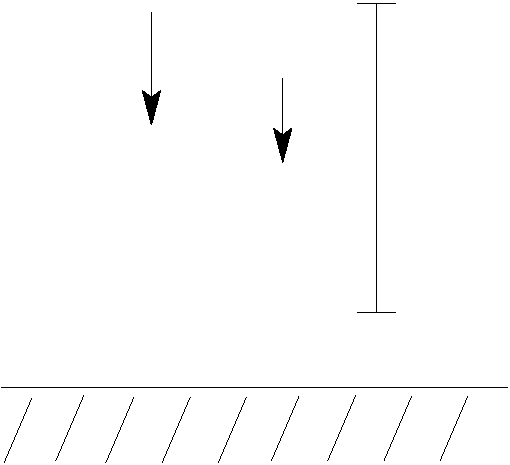
\includegraphics[height=12.7ex]{erde}}
		\put(11.0,17.2){\makebox(0,0)[l]{$A$}}
		\put(11.0, 8.5){\makebox(0,0)[l]{$B$}}
		\put( 7.8,16.0){\makebox(0,0){$m$}}
		\put( 3.5,15.0){\makebox(0,0)[r]{$g$}}
		\put(10.5,12.5){\makebox(0,0)[l]{$h$}}
		\put( 7.1, 4.0){\makebox(0,0)[t]{Earth}}
	\end{picture}
	%} %fbox
	\end{footnotesize}
	\caption{\label{fig:rotverschiebung}
		(a) Redshift by acceleration.
		(b) Redshift by gravitation.
	}
\end{figure}
%--- figure ----------------------------------------------------------
At time $t=0$, the lower observer sends a photon $\gamma$ in the direction of
the upper observer. Let us assume that the spacecraft is at rest at time $t=0$
relative to an initial system. Let $v=gt$ be the velocity of the two
observers after time $t$. Under the assumption $v \ll c$, we can
neglect terms of the order $v/c$ in the following approximation.
Then the photon reaches the upper observer in the time $t \approx h/c$.
Now the upper observer has reached the velocity $v = gt \approx gh/c$.
Due to the Doppler effect, he observes the photon with a redshift
\begin{equation}
	z := \frac{\Delta \lambda}{\lambda}
	\approx \frac{v}{c} \approx \frac{gh}{c^2}.
	\label{eq:rotverschiebung-1}
\end{equation}
According to the equivalence principle, the same redshift can also be expected for two observers
in a homogeneous gravitational field.
Since for a weak homogeneous gravitational field (such as on the Earth's surface)
$\Delta \Phi = gh$
applies to Newton's gravitational potential $\Phi$, we can also write Newton's approximation for the redshift
\begin{equation}
	z = \frac{\Delta \Phi}{c^2}
	.
	\label{eq:rotverschiebung-2}
\end{equation}
This formula could be confirmed up to 1\% by terrestrial experiments basing on the Möß\-bauer effect\index{Mößbauer effect}.

The redshift (\ref{eq:rotverschiebung-1}), however, also follows from the conservation of energy. Let us assume two points $A$ and $B$ in a homogeneous
gravitational field $g$ at a distance $h$ (Figure \ref{fig:rotverschiebung}b).
A mass $m$ falls from $A$ to $B$ with an initial velocity of 0.
At point $B$, according to Newton's theory, it has a kinetic energy
$E_{\mathrm{kin}} = mgh$. Now let us imagine that the entire energy
of the falling body, i.e., rest energy plus kinetic energy, is annihilated at point $B$
into a photon that moves back to point $A$ in the gravitational field.
If the photon had no interaction with the gravitational field, If the photon did not interact with the gravitational field,
we could convert it back into a mass $m$ there and would gain the energy $\Delta E = mgh$ in
this circular process.
In order to preserve the law of conservation of energy, the photon must therefore be shifted to the red. Therefore we obtain the following identities for the photon energy
$$
	E_{\mathrm{below}}
	= E_{\mathrm{above}} + mgh
	= mc^2 + mgh
	= mc^2 \left( 1 + \frac{gh}{c^2}\right)
	= E_{\mathrm{above}} \left( 1 + \frac{gh}{c^2}\right)
	.
$$
This means the the change of wave length
\begin{equation}
	1+z 
	= \frac{\lambda_{\mathrm{above}}}{\lambda_{\mathrm{below}}}
	= \frac{\hbar \omega_{\mathrm{below}}}{\hbar \omega_{\mathrm{above}}}
	= \frac{E_{\mathrm{below}}}{E_{\mathrm{above}}}
	= 1 + \frac{gh}{c^2}
	,
\end{equation}
coincides with (\ref{eq:rotverschiebung-1}).


\section{Exact vacuum solutions of the field equations}

Historically, the first exact solutions of the Einstein field equations with vanishing cosmological constant were found by Karl Schwarzschild in 1916 and by Alexander Friedmann in 1922. Schwarzschild's solution describes the gravitational field in a vacuum, enabling eventually the representation black holes, whereas Friedmann's solution represents a universe filled with a matter fluid of given density and pressure.
In this section we shortly consider the first one as a prominent vacuum solution. We return to Friedmann's solution below in chapter \ref{sec:FLRW-universes}.


%\subsection{Vacuum solutions}

The simplest class of exact solutions to Einstein's
field equations (\ref{eq:Feldgleichungen}), with $\Lambda = 0$, are the
\emph{vacuum solutions}\index{vacuum solutions}.
They solve the field equations with a vanishing
energy-momentum tensor, i.e.,
\begin{equation}
	T_{ij}
	= \left(\begin{array}{cccc}
		0   &   0   &   0   &  0 \\
		0   &   0   &   0   &  0 \\
		0   &   0   &   0   &  0 \\
		0   &   0   &   0   &  0
	\end{array}\right)
	.
	\label{eq:T-ij=0}
\end{equation}
The vacuum solutions thus represent gravitational fields in
a vacuum.
Since the field equations with (\ref{eq:T-ij=0}) are relatively
easy to solve, the first exact solutions to be discovered were two vacuum solutions:
the Minkowski space-time (by construction according to the equivalence principle, of course) and the Schwarzschild solution.


\subsection{Minkowski spacetime of special relativity}
The simplest solution to the field equation is the
\emph{Minkowski spacetime}\index{Minkowski spacetime}.
Its metric tensor in orthogonal coordinates $(t, x, y, z)$ is constant
\begin{equation}
	g_{ij}
	= \left(\begin{array}{@{}rrr@{\hspace*{3.5ex}}c}
		1   &   0   &    0   &  0 \\
		0   &  -1   &    0   &  0 \\
		0   &   0   &   -1   &  0 \\
		0   &   0   &    0   & -1
	\end{array}\right)
	.
	\label{eq:g-Minkoski}
\end{equation}
Since all derivatives of $g_{ij}$ disappear, space
and time are not curved.
In particular, light rays move in straight lines here,
but there is also no gravity.
Min\-kow\-ski space-time is the model of special
relativity.
Of course, Einstein knew this trivial solution
to his field equations; he had deliberately constructed his system of equations
in such a way that Minkowski spacetime would solve them,
cf. the correspondence principle above. However, for a non-vanishing cosmological constant this principle is not satisfied. \cite[151]{Straumann-1988}


\subsection{Black holes}
Einstein himself was unable to determine a non-trivial exact solution to his field equations.
But only a few months after their
publication, the astronomer Karl Schwarzschild succeeded in
finding the first exact solution to the complicated differential equations
for the case of a vacuum outside a given mass.
%It belongs to the class of \emph{vacuum solutions}\index{vacuum solution},
%It belongs to the class of \emph{vacuum solutions}\index{vacuum solution},
%i.e., the field equations for a vanishing energy-momentum tensor,
%\begin{equation}
%    T_{ij} = 0.
%\end{equation}
The solution found by Schwarzschild and now named after him
ultimately describes a black hole\index{black hole},
but this was not understood as a possible physical reality
until the 1960s. The metric tensor that solves the field equations has a
simple diagonal form
\begin{equation}
	g_{ij}
	= \left(\begin{array}{cccc}
		g_{tt} &   0    &   0    &  0     \\
		   0   & g_{rr} &   0    &   0    \\
		   0   &   0    & g_{\vartheta\vartheta} &  0 \\
		   0   &   0    &   0    & g_{\varphi\varphi} \\
	\end{array}\right)
	\label{eq:Schwarzschild-schema}
\end{equation}
and is usually described by the coordinates $(r, \vartheta, \varphi, ct)$,
where $t$ is time and 
$(r, \vartheta, \varphi)$
are the spatial spherical coordinates.
The  three spatial components of $g_{ij}$ have
a sign different from $g_{tt}$,
and the magnitude of the $g_{rr}$ component
is the reciprocal of the magnitude of $g_{tt}$,
\begin{equation}
	g_{rr} = -\frac{1}{g_{tt}}
    .
\end{equation}
In the 1960s, Kerr discovered an exact solution that generalized the Schwarzschild solution and contains non-vanishing
components in the secondary diagonal.
The Kerr solution represents a rotating gravitational source
in a vacuum. \cite[Chap. 6]{Chandrasekhar-1983} %\cite{de-Vries-2009}


%\subsection{Non-vacuum solutions: Models of the universe}
%
%The energy-momentum tensor 
%\begin{equation}
%	T_{ij}
%	= \left(\begin{array}{@{}rccc}
%	  \rho  &  0   &   0   &  0 \\
%		0   &  -p  &   0   &  0 \\
%		0   &  0   &  -p   &  0 \\
%		0   &  0   &   0   & -p \\
%	\end{array}\right)
%\end{equation}
%with two positive differentiable functions 
%$p = p(t)$ und $\rho = \rho(t)$
%represents physically an ideal fluid
%with pressure $p$ and energy density $\rho$.
%%As early as 1914, Einstein had described it as an example of a
%%non-vanishing energy-momentum tensor.
%With the “chronometric coordinates”
%$(\chi,\theta,\varphi, \tau)$, where 
%$(\chi,\theta,\varphi)$
%are spatial polar coordinates for $k \leqq 0$, similar to the Schwarzschild solution,
%and four-dimensional spherical coordinates for $k=1$
%\cite[§111]{Landau-Lifschitz-1997},
%as well as the differentiable functions $a = a(\tau)$ and
%\begin{equation}
%	f_k(\chi) = \left\{\begin{array}{@{\ }ll}
%        \sinh \chi & \mbox{for $k=-1$,} \\
%        \chi       & \mbox{for $k=0$,} \\
%        \sin \chi  & \mbox{for $k=1$.}
%    \end{array}\right.
%	\label{(3.23)}
%\end{equation}
%%In this section, we often write $f$ instead of $f_k$.
%we can then solve the field equations with the metric tensor
%\begin{equation}
%    g_{ij}
%	= a^2 \left(\begin{array}{@{\,}rccc}
%        1  &    0   &   0    &  0     \\
%        0  &   -1   &   0    &  0     \\
%        0  &    0   & -f_k^2 &  0     \\
%		0  &    0   &   0    & -f_k^2 \sin^2 \vartheta \\
%    \end{array}\right)
%    \label{eq:Robertson-Walker-Metrik}
%\end{equation}
%For more details, see, for example, \cite[§3.2]{de-Vries-1994}.
%%
%With the change of coordinates 
%%$(0, \infty) \times \tilde I_k \to (0, \infty) \times J_k$,
%$(\tau, \chi) \mapsto (t,r)$,
%\begin{equation}
%	\tau \mapsto t = \sigma(\tau), \qquad \chi \mapsto r = f_k(\chi),
%	\label{eq:Koordinatenwechsel}
%\end{equation}
%i.e., with
%\begin{equation}
%	\tau = \sigma^{-1}(t), \qquad
%	\chi = f_k^{-1}(r) = \left\{\begin{array}{@{\ }ll}
%		\mathrm{arsinh}\, r & \mbox{für $k=-1$,} \\
%		r & \mbox{für $k=0$,} \\
%		\arcsin\, r & \mbox{für $k=1$,}
%	\end{array}\right.
%	\label{(3.30)}
%\end{equation}
%and with the \emph{world radius}\index{world radius}
%\begin{equation}
%	R(t) := a\big(\sigma^{-1}(t)\big)\, /\, c,
%	\label{eq:def-R}
%\end{equation}
%$c$ the speed of light, we have
%\begin{equation}
%	\D \tau = \frac{c \D t}{R(t)}, \quad \mbox{bzw.} \quad c \D t = a(\tau) \D \tau, \qquad
%	\D\chi = \frac{\D r}{\sqrt{1 - kr^2}}\,.
%	\label{(3.32)}
%\end{equation}
%Therefore the metric reads
%\begin{equation}
%	\D s^2 = c^2 \D t^2 - R^2(t) 
%	\left( \frac{\D r^2}{1 - kr^2} + r^2 \D \theta^2 + r^2 \sin^2 \theta \D \varphi^2 \right).
%	\label{eq:Robertson-Walker}
%\end{equation}
%This is the \emph{Friedmann-Lemaître-Robertson-Walker} (FLRW) line element, the metric of a spactime that is obtained from the \emph{cosmological princip}\index{cosmological principle} of spacelike isotropy. \cite{Sexl-Urbantke-1987}, \cite[§5.3]{Hawking-Ellis-1973}.
%The parameter $t$ is the \emph{cosmic time}\index{cosmic time}.
%
%If, according to (\ref{eq:Koordinatenwechsel}), we only perform the coordinate transformation $\tau \mapsto t$, 
%then the line element of the metric tensor
%(\ref{eq:Robertson-Walker-Metrik}) with (\ref{eq:def-R}) for $k=1$ is
%\[
%	\D s^2 = c^2 \D t^2 - R^2(t) 
%	\left(\D \chi^2 + \sin^2 \chi \D\theta^2 + \sin^2\chi\sin^2 \theta \D\varphi^2 \right).
%\]
%The spatial part 
%$R^2(t) \left(\D \chi^2 + \sin^2 \chi \D\theta^2 + \sin^2\chi\sin^2 \theta \D\varphi^2 \right)$ 
%thus is exactly the three-dimensional line element of a hypersphere with radius $R$ embedded in Euclidian $\mathbb{R}^4$. This explains the designation “worl radius” for $R$. \cite[pp. 149]{Sexl-Urbantke-1987}.
%
%A physical model of the universe is obtained by
%substituting (\ref{eq:Robertson-Walker}) into Einstein's field equations with the energy-momentum tensor
%of an ideal fluid (“galactic gas”). This ultimately yields an
%ordinary nonlinear differential equation for $R(t)$, the \emph{Friedmann equation}
%\cite[pp.~156]{Sexl-Urbantke-1987}.
%%If $R(t)$ is a solution to this equation, the associated Robertson-Walker spacetime is called the \emph{Friedmann cosmos}.
%
% For  the  special  case  of  a  vanishing  cosmological constant
%(“vacuum energy density”), the Friedmann equation for a 
%matter-dominated  universe  (“incoherent”  or  “dust-like  matter”) reduces to the
%simple equation $(\D R/\D t)^2 = \mathscr{A}/R - k$, $\mathscr{A}$ $=$ const, which takes the form
%\[
%	(\dot{a})^2 = A_0 a - k a^2
%\]
%with $A_0 = \mathscr{A}/c^2$. \cite[p.~237]{Stephani-1991} 
%Separation of variables yields the solutions
%\begin{equation}
%	a(\tau) = \left\{ \begin{array}{@{\ }ll}
%		\frac12\, A_0 (\cosh \tau - 1) & \mbox{für $k = -1$,} \\[1.0ex]
%		\frac14\, A_0 \tau^2 & \mbox{für $k = 0$,} \\[1.0ex]
%		\frac12\, A_0 (1 - \cos \tau) & \mbox{für $k = 1$}
%	\end{array}\right.
%	\label{(3.34)}
%\end{equation}
%%mit $\tau \in I_k$. 
%By (\ref{eq:Koordinatenwechsel}) we then have 
%%$t = \frac{1}{c} \int a \D \tau$, d.h.\ $t \in J_k$,
%\begin{equation}
%	t = \left\{ \begin{array}{@{\ }ll}
%		\frac{1}{2c}\ A_0 (\sinh \tau - 1) & \mbox{für $k = -1$,} \\[1.0ex]
%		\frac{1}{12\,c}\ A_0 \tau^3 & \mbox{für $k = 0$,} \\[1.0ex]
%		\frac{1}{2c}\ A_0 (1 - \sin \tau) & \mbox{für $k = 1$.}
%	\end{array}\right.
%\end{equation}
%Since $a$ (except for a positive factor corresponding to the radius of the universe) describes the expansion of the universe,
%there are three different development scenarios depending on the parameter $k$, Fig. \ref{fig:Friedmann-Kosmen}.
%The first scenario $k = +1$ is the so-called “big crunch,” in which the universe collapses into a singularity after reaching its maximum expansion. This scenario is based on the assumption that the universe is finite and has a finite volume.
%\begin{figure}[htp]
%\centering
%\begin{footnotesize}
%\begin{tikzpicture}[>=stealth, domain=0:3.5, scale=0.4]
%	\draw[->] (-0.2,0) -- (11,0) node[right] {$t$};
%	\draw[->] (0,-.2) -- (0,7) node[left] {$a(t)$};
%	\draw[color=blue,thick]
%	plot ({sinh(0.9*\x) - 0.9*\x},{cosh(0.8*\x) - 1}) node[right] {$k = -1$};
%	\draw[color=gruen,thick]
%	plot ({.23*\x*\x*\x},{.45*\x*\x}) node[right] {$k = 0$};
%	\draw[color=rot,thick]
%	plot ({(3*\x - sin(150*\x))},{(1 - cos(150*\x))}) node[right] {$k = +1$};
%\end{tikzpicture}
%\hspace*{5ex}
%\begin{tabular}[b]{c}
%\begin{tikzpicture}[>=stealth, domain=0:3.5, scale=0.4]
%	\draw[->] (-2.0,0) -- (11,0) node[right] {$t$};
%	\draw[->] (0,-.2) -- (0,7) node[left] {$R(t)$};
%	\draw[color=gruen,thick]
%	plot ({.23*\x*\x*\x},{.55*\x*\x}) node[below] {$R(t)$};
%	\draw (-2,-.2) -- (9,7) node[left] {$h(t)$};
%	%\draw[circle (1ex)];
%	\draw[dashed] (3,-.2) -- (3,3); % node[left] {$R(t)$};
%	%\draw[dashed] (-1.7,-.2) -- (-1.7,3); % node[left] {$R(t)$};
%	\draw (3,0) node[below] {$t_0$}; % node[left] {$R(t)$};
%	\draw[|<->|,thick] (-1.7,3.5) --  node[above] {$\displaystyle \quad \frac{1}{H_0}$} (3,3.5);
%\end{tikzpicture}
%\\[-2.5ex]
%\end{tabular}
%\end{footnotesize}
%\caption{\label{fig:Friedmann-Kosmen}
%	Expansions of the three Friedmann cosmologies. The reciprocal of the Hubble constant $H_0$ represents an upper limit for the age of the universe, as can be seen from the tangent equation $h(t) = \dot{R}(t_0) (t-t_0) + R(t_0)$.}
%\end{figure}
%
%\noindent
%Also for a radiation-dominated Friedmann universe
%elementary solutions can be obtained for $\Lambda = 0$,
%cf. \cite[§26]{Stephani-1991}, 
%\cite[§5, especially pp. 156f and pp. 160ff]{Sexl-Urbantke-1987},
%\cite[p.~347ff]{O-Neill-1983},
%\cite[§§111--113]{Landau-Lifschitz-1997}.
%
%If we form the quotient of the derivative $\dot{R}$ of the world radius 
%and $R$, we obtain the relative rate of change of the universe
%\begin {equation}
%    H(t) = \frac{\dot{R}(t)}{R(t)}
%    ,
%\end{equation}
%the \emph{Hubble function} $H$.
%For the time $t_0$ $=$ now, $H_0$ $:=$ $H(t_0)$ 
%\emph{Hubble constant}\index{Hubble constant}.
%
%Its reciprocal $1/H_0$ indicates the maximum 
%age of the universe\index{age of the universe} for a non-accelerating
%expanding universe
%\cite{Sexl-Urbantke-1987}, because the equation of the tangent
%of the graph of $R(t)$ at the point $t_0$ is
%$h(t)$ $=$ $\dot{R}(t_0) (t-t_0) + R(t_0)$, 
%and its zero point is given by
%\begin{equation}
%	t_0 - t = \frac{R(t_0)} {\dot{R}(t_0)} = \frac{1}{H_0}
%\end{equation}
%given by \begin{equation}
%t_0 - t = \frac{R(t_0)} {\dot{R}(t_0)} = \frac{1}{H_0}
%\end{equation}
%see Figure \ref{fig:Friedmann-Kosmen}.
%
%Friedmann's models of the universe and more modern
%modifications such as the “inflationary universe” in its
%initial phase have repeatedly been confirmed by 
%physical observations. The first important
%confirmation was the discovery of the expansion of the universe
%
%Friedmann's models of the universe and more modern
%modifications such as the “inflationary universe” in its
%initial phase have repeatedly been confirmed by 
%physical observations. The first important
%confirmation was the discovery of the expansion of the universe
%by the Belgian priest and astrophysicist Georges Lemaître
%in 1927 \cite{Lemaitre-1927} and the US astronomer
%Edwin Hubble in 1929 \cite{Hubble-1929}.
%Further confirming observations were
%the discovery of cosmic background radiation by
%Penzias and Wilson in 1965 and the discovery of the Higgs boson
%in 2012, cf.
%\cite[§20.1]{Karttunen-et-al-2000},
%\cite[§13.3]{Unsoeld-Baschek-1999}


\section{General relativity in everyday life}
Most of the most important applications of general relativity are, naturally, in astronomy, especially
astrophysics and cosmology. After all, 
considerable gravitational fields or space and time scales are required to observe or utilize relativistic effects.
In everyday life, one would not expect Einstein's
hundred-year-old field equations to have any impact or even
significance at all.
After all, it is not exactly common to have a black hole in one's
handbag or a small inflationary universe in one's
closet.
And warp drive, which would allow one to travel to the nearest wormhole around the corner, is not yet functional.
It is therefore all the more surprising that there are indeed very practical
This makes it all the more astonishing that there are indeed very practical
applications and explanations of the general theory of relativity that 
affect our everyday lives.


\subsection{Olbers' paradox}
%\section{Der Himmel ist dunkel}
For a long time, it was an unexplained phenomenon that the sky is dark at night.
Olbers' paradox\index{Olbers' paradox} 
states the following:

\begin{satz}[\textbf{Olbers' paradox (1823) \cite{Olbers-1826}}]
	If the universe is infinite and uniform in space and time
    and filled with stars like our sun, 
    then the sky is at least
    as bright as the average luminosity $L$ of the stars everywhere.
	%\cite[§13.2.6]{Unsoeld-Baschek-1999}
\end{satz}
\begin{proof}
	\cite{Tipler-1988}
	Each spherical shell with radius $r$ and thickness $\D r$ around the Earth
    contains $4 \pi \rho r^2 \D r$ stars, where $\rho$ denotes the average star density.
    The apparent luminosity of a star on Earth is
    $L/r^2$.
	Therefore, each spherical shell 
    radiates with an apparent luminosity of $4 \pi \rho L \D r$.
    This integrand is constant and, in particular, independent of $r$.
%    The stars closer to Earth can absorb light sources behind them,
%    but due to the conservation of energy,
%    they must ultimately re-emit this energy.
\end{proof}

%\noindent
But why is it dark at night?
At least one of the three premises of the sentence must be false
so that it does not contradict our observations.
Either the universe is finite in space or time 
(or both),
or it is not uniformly filled with sun-like stars.
Einstein's field equations provide, for the first time in the
history of science, physically testable %quantifiable 
cosmological models
that solve Olbers' paradox by allowing for a temporally finite
universe.


\subsection{GPS}
GPS (Global Positioning System, officially NAVSTAR GPS) is a global satellite-based navigation system for determining position. To do this, the satellites constantly transmit their current position and the exact time using coded radio signals. GPS receivers can then calculate their own position and speed from the signal transit times. In theory, signals from three satellites with simultaneous radio contact are sufficient for this. 
%--- Figure: -----------------------------------------------------------
\begin{figure}[htp]
\centering
	\includegraphics[height=30ex]{GPS}
	\caption{\label{fig:GPS}
		Satellite-based navigation systems such as GPS
		(Source:
		\url{https://tug.org/TUGboat/tb33-1/tb103wolcott.pdf})
	}
\end{figure}
%--- Figure ------------------------------------------------------------
However, since GPS receivers do not necessarily use an accurate clock to measure the transit time, the signal from a fourth satellite is required to determine the exact time in the receiver.
GPS was launched in February 1978 and is based on 31 satellites.

A physical system rotating in a circular orbit around a static spherically symmetric 
gravitational field of mass $M$ can be described in general relativity by
the Schwarzschild metric \cite{de-Vries-1994,de-Vries-1996} 
with $\D r$ $=$ $\D \varphi$ $=$ $0$,
\begin{equation}
	\D s^2
	= c^2 \D \tau^2
	= \left(1 - \frac{2GM}{c^2 r}\right) c^2 \D t^2 - r^2 \D \vartheta^2
	.
\end{equation}
Here, $\tau$ denotes the proper time of the rotating system.
($t$ denotes the coordinate time of the entire gravitational field
and corresponds to the proper time of a stationary observer at infinity,
$r \to \infty$.)
It follows that
\begin{equation}
	\Big(\frac{\D \tau}{\D t}\Big)^2
	= \left(1 - \frac{2GM}{c^2 r}\right) 
	- \frac{r^2}{c^2} \, \frac{\D \vartheta}{\D t}
	= 1 + \frac{2 \Phi(r)}{c^2} - \frac{v^2}{c^2}
\end{equation}
with the gravitational potential $\Phi(r)$ 
%Relativitätstheorie $g_{44} = 1 - \Phi/c^2$
\cite[VI.2]{Straumann-1988}. %S. 261
and the orbital speed
$v(r)$ given by
\begin{equation}
	\Phi(r)
	= - \frac{M G}{r}
	, \qquad
	v(r) = r \, \frac{\D \vartheta}{\D t}
\end{equation}
This results in the proper times $\tau_E$ and $\tau_S$ of a receiver
on Earth with Earth radius $r_E$ and a satellite orbiting the Earth in a circular orbit
with radius $r_S$
\cite{Pascual-Sanchez-2007}
\begin{equation}
	\Big(\frac{\D \tau_S}{\D \tau_E} \Big)^2
	= \frac{1 + 2\Phi(r_S)/c^2 - v_S^2/c^2}
		{1 + 2\Phi(r_E)/c^2 - v_E^2 / c^2}
	\label{eq:GPS-Eigenzeiten}
\end{equation}
Since the gravitational field of the Earth is quite small on the Earth's surface,
 i.e., $\Phi(r_E)/c^2 \ll 1$, and since the velocities
$v_E$ and $V_S$ are much smaller than the speed of light,
the approximation
can be applied for equation (\ref{eq:GPS-Eigenzeiten}),
neglecting terms higher than $O(c^{-2})$, \cite{Pascual-Sanchez-2007,Singer-1956}.
\begin{equation}
	\frac{\D \tau_S}{\D \tau_E}
	= \frac{\sqrt{1 + 2\Phi(r_S)/c^2 - v_S^2/c^2}}
		{\sqrt{1 + 2\Phi(r_E)/c^2 - v_E^2 / c^2}}
	= %\approx
	1 + \frac{MG}{c^2} \left(\frac{1}{r_E} - \frac{1}{r_S}\right)
	+ \frac{v_E^2 - v_S^2}{2\, c^2}
	+ O(c^{-3})
	\label{eq:GPS-Zeitdilatation-approx}
\end{equation}
With the difference $\Delta \Phi = \Phi(r_E) - \Phi(r_S)$
between the two gravitational potentials and the difference
$\Delta v^2$ between the squares of the velocities,
\begin{equation}
	\Delta \Phi
	= {M G}
	\left(\frac{1}{r_E} - \frac{1}{r_S}\right)
	,
	\qquad
	\Delta v^2 = v_S^2 - v_E^2
	\label{eq:GPS-Potentialdifferenz}
\end{equation}
we thus have
\begin{equation}
	\frac{\D \tau_S}{\D \tau_E}
	\approx
	1 + \frac{\Delta \Phi}{c^2} - \frac{\Delta v^2}{2\,c^2}
	.
	\label{eq:GPS-Zeitdilatation}
\end{equation}
See \cite[Gl. (14.12)]{Sonne-Weiss-2013}.
This means that the time displayed by the atomic clocks on the GPS satellites is subject to special relativistic \emph{and} gravitational time dilation. According to general relativity, the rate at which a clock runs depends on its location in the gravitational field,
i.e., on $\Delta \Phi$, 
and according to special relativity, it depends on its velocity $v_S$.
The lower gravitational potential in the satellite's orbit causes time to pass more quickly than on Earth, while the orbital motion of the satellites relative to a stationary observer on Earth slows it down.
The two time dilations therefore have opposite effects.
In other words, for an observer on the Earth's surface, 
time passes 
slower than for an observer on the satellite, who is not moving relative to him, 
by a factor of $1 + \frac{\Delta \Phi}{c^2}$.

For the values
$M = 5.98 × 10^{24}$ kg, 
$r_E = 6.38 × 10^{6}$ m
and $r_S = 26.56 × 10^{6}$ m,
 equation (\ref{eq:GPS-Potentialdifferenz}) yields
$\Delta \Phi/c^2 = 5.28 \cdot 10^{-10}$
and
$\Delta v^2 = 8.5 \cdot 10^{-11}$ m/s.
In the GPS satellite orbit, the gravitational effect therefore predominates 
by more than six times: time therefore passes faster on the satellites. 
Equation (\ref{eq:GPS-Zeitdilatation}) yields
the relative satellite velocity $v_S = 3900$ m/s
and the relative rate difference  
\begin{equation}
	\frac{\D \tau_S}{\D \tau_E}
	= 1 + 4{,}44 \cdot 10^{-10}
\end{equation}
the proper times on Earth and in the satellite.
This ratio is significantly greater than the relative accuracy of cesium atomic clocks, which is of the order of $10^{-13}$.
To compensate for this time dilation, the oscillation frequency
of the satellite clocks is detuned to $\mu_{S}$ $=$ 10.229999995453 MHz, 
so that they always run synchronously with the frequency $\mu_{E}$ $=$ 10.23 MHz
of the terrestrial receiver clocks.
(The sample actually yields $\mu_E/\mu_S - 1 = 4.44 \cdot 10^{-10}$.)

If time dilation were not compensated for, the
difference in the rate of the clocks per year would add up to a time difference
of % between satellite clocks and clocks on Earth 
of approximately 0{,}014 seconds.
Accordingly, time dilation would lead to a deviation
\begin{equation}
	\frac{\D s}{\D \tau_E} - c
	= c \left(\frac{\D \tau_S}{\D \tau_E} - 1\right)
	= 0{,}133 \mbox{ m$/$s}
\end{equation}
Per second, the car would deviate 13 cm from its calculated
course, or 8 meters per minute or 11.5 km per day.
However, this error would not occur even without the corrective adjustment
of the satellite clocks in the real GPS system, because
at least four satellites are always contacted to determine time and location, so that only the satellite time is actually used.

%
At an altitude of about 3,000 km, 
special relativistic and gravitational time dilation
cancel each other out.
